\phantomsection %% non so perché senza l'indice funziona male :///
% -------------------------------------------------------
\section{Architecture Choice and Language Used}
% -------------------------------------------------------
This section aims to provide a clear description of the architecture and language used in the developement of the HealthMaxxing app. Together with the reasons behind such choices.
\phantomsection 
\subsection{Architecture Type: 3-Tier Architecture}
\phantomsection 
\subsubsection{Description}

The application follows a \textbf{3-Tier Architecture} pattern, separating the system into three distinct layers:

\begin{itemize}
  \item \textbf{Presentation Layer (Frontend)} --- React with Vite
  \item \textbf{Business Logic / API Layer (Backend)} --- Django REST Framework
  \item \textbf{Data Layer (Database)} --- PostgreSQL
\end{itemize}
\phantomsection 
\subsubsection{Why 3-Tier?}

\begin{itemize}
  \item \textbf{Maintainability:} Each tier can be developed, tested, and maintained independently. Changes in one layer do not directly affect others.
  \item \textbf{Separation of Duties:} Clear separation between UI concerns, business logic, and data persistence. Frontend developers focus on UX, backend developers focus on APIs and business rules, and database administrators manage data integrity.
  \item \textbf{Scalability:} Each tier can be scaled independently based on demand. The frontend can be served via CDN, the API can be load-balanced, and the database can use replication.
  \item \textbf{Industry Standard:} 3-tier is the most widely adopted pattern in modern web development, making the codebase more familiar to new team members.
\end{itemize}

\phantomsection 
\subsubsection{Project Structure}

\textbf{Main folders and files:}

\begin{itemize}
    \item \textbf{backend/} --- Contains the Django REST Framework application, business logic, models, serializers, and API endpoints.
    
    \item \textbf{frontend/} --- Contains the React application, user interface components, routing, state management, and API integration.
    
    \item \textbf{nginx/} --- Configuration files for the Nginx reverse proxy.
    
    \item \textbf{docs/} --- Project documentation and supporting materials.
    
    \item \textbf{docker-compose.yml} --- Defines and orchestrates the multi-container application environment.
    
    \item \textbf{Dockerfile.devbox} --- Docker image configuration used during development.
    
    \item \textbf{requirements.txt} --- Python dependencies required by the backend.
    
    \item \textbf{package.json} --- JavaScript dependencies and scripts used by the frontend.
    
    \item \textbf{README.md} --- General project documentation and setup instructions.

    \begin{figure}[htbp]
      \centering
      
\includegraphics[width=0.35\textwidth]{ScreenshotD3/FoldStruct.jpeg}
      \caption{Project structure}
      \label{fig:folder-structure}
    \end{figure}
    \FloatBarrier

\end{itemize}
\phantomsection 
% -------------------------------------------------------
\subsection{Language Used and Why}
% -------------------------------------------------------
\phantomsection 
\subsubsection{Frontend Language: JavaScript (React 18.3.1)}

\textbf{Why React?}

\begin{itemize}
  \item \textbf{Reusable Components:} React's component-based architecture allows building modular, reusable UI pieces that reduce code duplication.
  \item \textbf{Flexibility for Routing:} React Router DOM enables client-side routing, allowing seamless navigation without full page reloads.
  \item \textbf{Security Measures:} React provides built-in protections against common vulnerabilities like XSS attacks through automatic escaping.
  \item \textbf{Large Ecosystem:} Extensive community support, libraries, and tools available.
  \item \textbf{Developer Experience:} JSX syntax makes code more readable and maintainable.
\end{itemize}

\textbf{Why NOT Plain HTML/CSS?}

\begin{itemize}
  \item Plain HTML/CSS is considered outdated for modern web applications and not an industry standard.
  \item Lacks dynamic interactivity without extensive custom JavaScript.
  \item No component reusability or state management capabilities.
  \item Poor performance with complex UIs.
\end{itemize}
\phantomsection 
\subsubsection{Backend Language: Python (Django 4.2.30)}

\textbf{Why Django?}

\begin{itemize}
  \item Included as the framework of choice for this project.
  \item Excellent for rapid API development with built-in authentication, ORM, and admin panel.
  \item Strong security features (CSRF protection, SQL injection prevention, etc.).
  \item Well-documented and widely used in production environments.
\end{itemize}
\phantomsection 
% -------------------------------------------------------
\subsection{Database: PostgreSQL}
% -------------------------------------------------------
\phantomsection 
\subsubsection{Why PostgreSQL?}

\begin{itemize}
  \item \textbf{Team Familiarity:} All team members are comfortable with PostgreSQL and the relational database paradigm.
  \item \textbf{Industry Standard:} PostgreSQL is a robust, production-ready relational database trusted by many organizations.
  \item \textbf{Strong Consistency:} ACID compliance ensures data integrity.
  \item \textbf{Advanced Features:} Supports JSON, full-text search, and complex queries out of the box.
\end{itemize}
\phantomsection 
\subsubsection{ER Diagram}

\begin{figure}[htbp]
    \centering
    \includegraphics[width=\textwidth]{ScreenshotD3/ER.png} % Scales to exactly 100% of text width
    \caption{ER diagram}
    \label{fig:large_image}
\end{figure}

\FloatBarrier
\phantomsection 
\subsubsection{Example of some Tables}

\begin{figure}[htbp]
        \centering
        \begin{subfigure}[b]{0.47\textwidth}
            \centering
            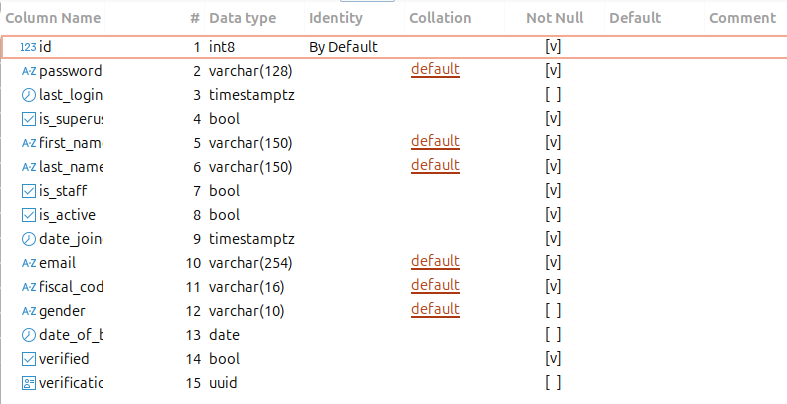
\includegraphics[width=\linewidth]{ScreenshotD3/tableUser.png}
            \caption{}
            \label{User Table}
        \end{subfigure}
        \hfill \begin{subfigure}[b]{0.47\textwidth}
            \centering
            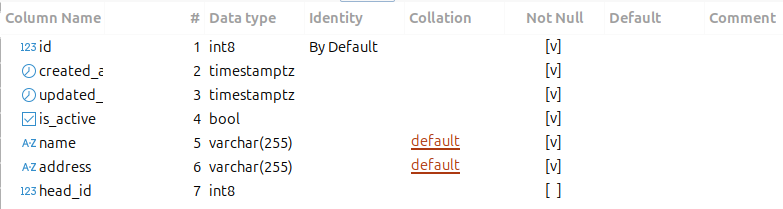
\includegraphics[width=\linewidth]{ScreenshotD3/tableHospital.png}
            \caption{}
            \label{Hospital Table}
        \end{subfigure}
        
        \caption{table of users (a), table of hospitals (b)}
        \label{User and Hospital Tables}
\end{figure}
\FloatBarrier

\phantomsection 
% -------------------------------------------------------
\subsection{Dependencies}
% -------------------------------------------------------
\phantomsection 
\subsubsection{Backend Dependencies}

\begin{longtable}{L{3.6cm} C{2.0cm} L{8.8cm}}
  \rowcolor{tableheader}
  \color{white}\bfseries Dependency &
  \color{white}\bfseries Version &
  \color{white}\bfseries Purpose \\
  \endfirsthead
  \rowcolor{tableheader}
  \color{white}\bfseries Dependency &
  \color{white}\bfseries Version &
  \color{white}\bfseries Purpose \\
  \endhead
  Django & 4.2.30 & Core web framework used to build the backend application and REST API \\
  \rowcolor{tablerowalt}
  Django REST Framework & 3.17.1 & Provides tools for building RESTful APIs, including serialization, authentication, and viewsets \\
  django-admin-confirm & 1.0.1 & Adds confirmation steps to Django admin actions to prevent accidental bulk operations \\
  \rowcolor{tablerowalt}
  django-cors-headers & 4.9.0 & Handles Cross-Origin Resource Sharing (CORS) between frontend and backend services \\
  djangorestframework-simplejwt & 5.5.1 & Implements JWT-based authentication for Django REST Framework \\
  \rowcolor{tablerowalt}
  psycopg & 3.3.4 & PostgreSQL database adapter for Python \\
  psycopg-binary & 3.3.4 & Pre-compiled PostgreSQL adapter for simplified installation and development \\
  \rowcolor{tablerowalt}
  ruff & 0.15.14 & Python linter and formatter used to enforce code quality standards \\
  asgiref & 3.11.1 & ASGI utilities providing asynchronous support required by Django \\
  \rowcolor{tablerowalt}
  sqlparse & 0.5.5 & SQL parsing library used internally by Django \\
  typing\_extensions & 4.15.0 & Backported and experimental type hinting features for Python \\
  \rowcolor{tablerowalt}
  tzdata & 2026.2 & Time zone database used for accurate date and time handling \\
  PyJWT & 2.13.0 & Creates, signs, decodes, and validates JSON Web Tokens \\
\end{longtable}
\phantomsection 
\subsubsection{Frontend Dependencies}

\begin{longtable}{L{3.6cm} C{2.0cm} L{8.8cm}}
  \rowcolor{tableheader}
  \color{white}\bfseries Dependency &
  \color{white}\bfseries Version &
  \color{white}\bfseries Purpose \\
  \endfirsthead
  \rowcolor{tableheader}
  \color{white}\bfseries Dependency &
  \color{white}\bfseries Version &
  \color{white}\bfseries Purpose \\
  \endhead
  React & 18.3.1 & Core UI library for building interactive components \\
  \rowcolor{tablerowalt}
  react-dom & 18.3.1 & Renders React components to the DOM \\
  react-router-dom & 6.0.0 & Client-side routing for seamless page navigation \\
  \rowcolor{tablerowalt}
  react-big-calendar & 1.20.0 & Feature-rich calendar component for displaying and managing scheduled events \\
  Vite & 5.4.1 & Lightning-fast build tool and dev server (modern webpack alternative) \\
  \rowcolor{tablerowalt}
  @vitejs/plugin-react & 4.3.1 & Vite plugin for React support with Fast Refresh \\
  axios & 1.17.0 & Promise-based HTTP client for making API requests from the frontend \\
  \rowcolor{tablerowalt}
  date-fns & 4.4.0 & Lightweight utility library for parsing, formatting, and manipulating dates \\
  zustand & 5.0.14 & Lightweight state management library for global application state, including authentication data \\
  \rowcolor{tablerowalt}
  jwt-decode & 4.0.0 & Decodes JWT tokens on the client side to extract user information and token claims without server requests \\
\end{longtable}
\phantomsection 
\subsubsection{Infrastructure Dependencies}

\begin{longtable}{L{3.6cm} L{10.8cm}}
  \rowcolor{tableheader}
  \color{white}\bfseries Dependency &
  \color{white}\bfseries Purpose \\
  \endfirsthead
  \rowcolor{tableheader}
  \color{white}\bfseries Dependency &
  \color{white}\bfseries Purpose \\
  \endhead
  Nginx & Reverse proxy server for routing requests, serving static assets, and load balancing \\
  \rowcolor{tablerowalt}
  Docker & Containerization platform for consistent development, testing, and production environments \\
  docker-compose & Orchestrates multi-container Docker applications (frontend, backend, database) \\
\end{longtable}

\textbf{Why These Infrastructure Tools?}

\begin{itemize}
  \item \textbf{Nginx:} Acts as a reverse proxy, routing frontend requests to the React app and API requests to Django. Improves performance and security.
  \item \textbf{Docker:} Ensures the application runs consistently across all environments (local, CI/CD, production). Eliminates ``works on my machine'' problems.
  \item \textbf{docker-compose:} Simplifies local development by defining and running all services (frontend, backend, database) in one configuration file.
\end{itemize}

\phantomsection
\subsubsection{Infrastructure Implementation}

The project's infrastructure is orchestrated using Docker Compose, which defines a unified, isolated, and easily reproducible development environment. Instead of running services directly on the host machine, the infrastructure is containerized into four distinct interconnected services under a shared custom network (\texttt{health-maxxing-network}).

The implemented services are structured as follows:

\begin{itemize}
    \item \textbf{Database (\texttt{db})}:
    \begin{itemize}
        \item Runs a PostgreSQL 16 instance based on an Alpine Linux image to keep the footprint minimal.
        \item Utilizes a dedicated Docker volume (\texttt{postgres-data}) mapped to the container's internal storage, ensuring that database records are preserved across container restarts and rebuilds.
        \item Includes an automated health check to verify that the database is fully ready to accept connections before dependent services start up.
    \end{itemize}
    
    \item \textbf{Development Workspace (\texttt{devbox})}:
    \begin{itemize}
        \item Acts as the central execution environment, built from a custom \texttt{Dockerfile.devbox}.
        \item The entire local project directory is mounted into the container as a volume, allowing real-time code synchronization between the host and the container.
        \item It manages the runtime for both the Django backend (port 8000) and the React frontend (port 3000). It is strictly configured to wait for the \texttt{db} to be healthy and the \texttt{mail} service to be started before initializing.
    \end{itemize}
    
    \item \textbf{Reverse Proxy (\texttt{nginx})}:
    \begin{itemize}
        \item An Nginx 1.27 container that acts as the entry point for external traffic on port 8080.
        \item It loads a custom routing configuration (\texttt{default.conf}) to properly direct requests to either the frontend or backend services running inside the \texttt{devbox}.
    \end{itemize}
    
    \item \textbf{Mail Service (\texttt{mail})}:
    \begin{itemize}
        \item Utilizes Mailpit to capture and inspect outgoing emails during development.
        \item It exposes port 1025 for internal SMTP routing (used by the Django backend) and port 8025 for a web-based user interface where developers can review the intercepted emails without sending them to real addresses.
    \end{itemize}
\end{itemize}

\phantomsection 
% -------------------------------------------------------
\subsection*{Summary}
% -------------------------------------------------------

\begin{tabular}{L{2.6cm} L{3.4cm} L{7.4cm}}
  \rowcolor{tableheader}
  \color{white}\bfseries Component &
  \color{white}\bfseries Choice &
  \color{white}\bfseries Reason \\
  Architecture & 3-Tier & Maintainability, separation of duties, scalability \\
  \rowcolor{tablerowalt}
  Frontend & React 18 + Vite & Reusable components, flexible routing, security, modern tooling \\
  Backend & Django + DRF & Rapid API development, built-in security, ORM, admin panel \\
  \rowcolor{tablerowalt}
  Database & PostgreSQL & Team familiarity, relational paradigm, ACID compliance, industry standard \\
  Infrastructure & Docker + Nginx & Consistency, reverse proxy, containerization, ease of deployment \\
\end{tabular}